\documentclass[aspectratio=169,11pt]{beamer}
\usepackage[T1]{fontenc}
\usepackage{amsmath,amssymb}
\usepackage{graphicx}
\usepackage{booktabs}

% Look: change the theme or the colour here.
\usetheme{Madrid}
\usecolortheme{default}
\definecolor{accent}{HTML}{1F5F8B}
\setbeamercolor{structure}{fg=accent}
\setbeamertemplate{navigation symbols}{}
\setbeamertemplate{caption}[numbered]

% Replace with your title, name, affiliation and date.
\title[Occupancy Sensing at the Edge]{Low-Power Occupancy Sensing for Smart Buildings}
\subtitle{Edge-Deployed Neural Networks on Battery-Powered Sensor Nodes}
\author[P. Raman]{Priya Raman \and Daniel Okafor \and Mei Tanaka}
\institute[Northfield]{Northfield Institute of Technology \and Harbour Automation Ltd.}
\date{Smart Buildings Workshop, 14 March 2026}

% Shows the outline again at the start of every section. Delete this block to turn that off.
\AtBeginSection[]{
  \begin{frame}{Outline}
    \tableofcontents[currentsection]
  \end{frame}
}

\begin{document}

\begin{frame}
  \titlepage
\end{frame}

\begin{frame}{Outline}
  \tableofcontents
\end{frame}

\section{Motivation}

\begin{frame}{Most rooms are empty most of the time}
  \begin{itemize}
    \item Ventilation and lighting run on fixed schedules, from early morning until evening.
    \item Meeting rooms in our building were occupied for only \textbf{31\%} of scheduled hours.
    \item Knowing \emph{whether} and \emph{by how many} people a room is used lets the controller match supply to demand.
  \end{itemize}
  \vspace{1em}
  \begin{block}{Question}
    Can a battery-powered sensor node estimate occupancy accurately enough to control ventilation?
  \end{block}
\end{frame}

\begin{frame}{Why not a camera or a motion detector?}
  \begin{columns}[T]
    \begin{column}{0.48\textwidth}
      \textbf{Cameras}
      \begin{itemize}
        \item Accurate counts
        \item Privacy concerns
        \item Need mains power and cabling
      \end{itemize}
    \end{column}
    \begin{column}{0.48\textwidth}
      \textbf{Motion detectors}
      \begin{itemize}
        \item Cheap and private
        \item Miss people sitting still
        \item Cannot count
      \end{itemize}
    \end{column}
  \end{columns}
  \vspace{1.2em}
  \centering
  Our approach: combine three inexpensive sensors \alert{on the node itself}.
\end{frame}

\section{Method}

\begin{frame}{The sensor node}
  \begin{figure}
    \centering
    % Replace with your own figure: upload an image and change the file name below.
    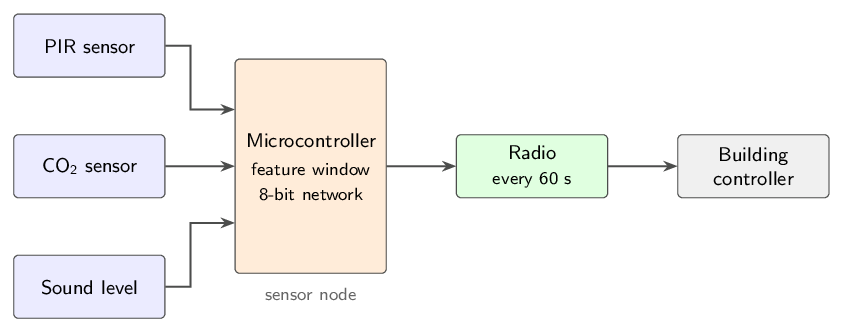
\includegraphics[width=0.82\textwidth]{figures/system-overview.png}
    \caption{Three sensors feed a small neural network; only the estimate leaves the room.}
  \end{figure}
\end{frame}

\begin{frame}{Model and training objective}
  \begin{itemize}
    \item Input: one minute of readings from each sensor, a $3 \times 60$ window $\mathbf{x}$.
    \item Two depthwise-separable convolution layers, 4.1 thousand parameters.
    \item An empty room mistaken for an occupied one costs more than a miscount:
  \end{itemize}
  \begin{equation}
    \mathcal{L}(\theta) = -\frac{1}{N} \sum_{i=1}^{N} w_{y_i} \log p_\theta(y_i \mid \mathbf{x}_i) + \lambda \lVert \theta \rVert_2^2
  \end{equation}
  \begin{itemize}
    \item Weights $w_0 = 2$ for the empty class, $w_c = 1$ otherwise.
  \end{itemize}
\end{frame}

\begin{frame}{Making it fit on a microcontroller}
  \begin{enumerate}
    \item<1-> Train for 40 epochs in floating point.
    \item<2-> Constrain weights and activations to 8-bit integers.
    \item<3-> Train for 10 more epochs so the model adapts to rounding.
  \end{enumerate}
  \vspace{1em}
  \onslide<3->{
    \begin{alertblock}{Result}
      38 ms per inference, 0.31 mW on average, 3.4 years on two AA cells.
    \end{alertblock}
  }
\end{frame}

\section{Results}

\begin{frame}{Accuracy on four rooms the model had not seen}
  \begin{table}
    \centering
    \begin{tabular}{lccc}
      \toprule
      Method & Detection (\%) & Count $\pm 1$ (\%) & Power (mW) \\
      \midrule
      PIR with timeout       & 83.3 & --   & 0.12 \\
      Boosted trees (server) & 90.6 & 79.4 & 4.80 \\
      Ours, floating point   & 95.1 & 88.9 & 0.74 \\
      \textbf{Ours, 8-bit}   & \textbf{94.2} & \textbf{87.6} & \textbf{0.31} \\
      \bottomrule
    \end{tabular}
    \caption{Twelve weeks, 14 meeting rooms, four held out for testing.}
  \end{table}
\end{frame}

\begin{frame}{Quantization costs less than one point of accuracy}
  \begin{columns}[c]
    \begin{column}{0.56\textwidth}
      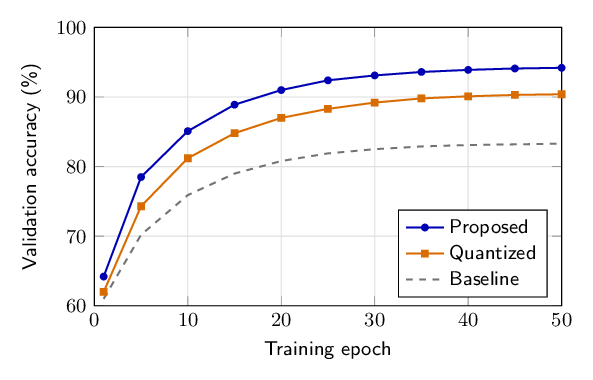
\includegraphics[width=\textwidth]{figures/accuracy.png}
    \end{column}
    \begin{column}{0.4\textwidth}
      \begin{itemize}
        \item Proposed model: 95.1\%
        \item After 8-bit quantization: 94.2\%
        \item Baseline: 83.3\%
      \end{itemize}
    \end{column}
  \end{columns}
\end{frame}

\begin{frame}{Energy saved in the building}
  \begin{itemize}
    \item Estimates controlled ventilation in 7 rooms for four weeks; 7 rooms kept the schedule.
    \item Fan energy in controlled rooms: \textbf{23\% lower}.
    \item Carbon dioxide below 1000 ppm for 99.1\% of occupied time (schedule: 99.4\%).
  \end{itemize}
  \vspace{1em}
  \begin{exampleblock}{Savings per room}
    \[
      E_{\text{saved}} = (1 - 0.77) \times 4.6\ \text{kWh/week} \approx 1.1\ \text{kWh/week}
    \]
  \end{exampleblock}
\end{frame}

\section{Conclusion}

\begin{frame}{Summary and next steps}
  \begin{itemize}
    \item A 4.1k-parameter network on a battery-powered node detects occupancy with 94.2\% accuracy.
    \item The node draws 0.31 mW and only an estimate leaves the room.
    \item Ventilation controlled by the estimates used 23\% less fan energy.
  \end{itemize}
  \vspace{1em}
  \textbf{Next:} a full heating season, and open-plan areas.
\end{frame}

\begin{frame}
  \centering
  {\Huge Thank you}\\[1.5em]
  {\large Questions?}\\[2em]
  Priya Raman\\
  \texttt{priya.raman@northfield.example}
\end{frame}

\end{document}
